\documentclass{article}
\usepackage{enumitem}
\usepackage{graphicx}
\usepackage[utf8]{inputenc}
\usepackage{listings, xcolor}
\usepackage[hyphens,spaces,obeyspaces]{url}
\usepackage{placeins}




\graphicspath{ {./pictures/} }

\author{Kenneth Hansen - cph-kh415@cphbusiness.dk
    \and Martin Høigaard Cupello - cph-mr221@cphbusiness.dk}

\title{Supervised Classifiers Comparison} 


\begin{document}
\maketitle
\thispagestyle{empty}

\begin{abstract}
  \noindent It is difficult to decide on which supervised machine learning classification model to implement on a dataset.
  This can be problem since choosing the wrong model may lead to inaccurate predictions.
  This article will compare a selection of models to determine which model is the most accurate.
  This would help on deciding which model to apply to a given classification dataset.
\end{abstract}
\tableofcontents
\clearpage



\section{Introduction}
This article will compare different machine learning classifiers, and try to determine which one is the most accurate for supervised classification. We will use the popular iris dataset to test different supervised machine learning algorithms, collect metrics, and finally test our findings against two other datasets to see if the results can be confirmed and compare accuracy scores to find the most accurate model.

\bigskip

\noindent Our hypothesis is that there exists a single classification model which provides the most accurate predictions on all datasets.

\section{Supervised learning}
Supervised learning is a type of artificial intelligence and also a machine learning algorithm. The algorithm takes an input variable x and an output y, to learn how the input gets the desired output Y = f(X). This is normally done with a training dataset to produce an accurate prediction. It can be divided into two groups: Classification, where the model assigns a category based on the given input,  and regression, which is used to understand the relationship between dependent and independent variables.

\noindent This article will be comparing classification models.

\subsection{KNN}
KNN (K Nearest Neighbor) tries to determine which group the data belongs to, based on proximity to the nearest neighbors.
KNN does not make any assumptions; it only uses input data which makes an educated guess of the output based on its closest neighbors.
How to choose K:
A good estimate to choose K is to take the square root of n, where n is the size of your training data. However, depending on the size of the dataset, it might not be the best.

\subsection{Gaussian Naive Bayes and Multinomial Naive Bayes}
These classifiers are called “probabilistic classifiers” and use statistics by adding the probability of each input parameter to determine which category the data is most likely to belong to. They are called “naive” since they all treat variables as independent of each other, but they use different algorithms to predict the result.
The gaussian naive bayes uses a gaussian distribution, where the probability is calculated using the standard deviation and mean for each input.
The multinomial naive bayes assumes that all distributions are multinomial, which means more than 2 input variables.


\subsection{Decision Tree}
The decision tree is a tree-like structure consisting of nodes and branches. The root node is the starting point which is the entire dataset. Then the node is split into decision nodes, based on the labels attributes.
At the end of the tree are the terminal nodes which are the labels/classifications. 
This is better explained by using the picture below. Assume there is a dataset consisting of animal attributes. You are trying to determine the type/species of an animal, based on its attributes. First the model ask if it has feathers, and based on this decision node, the tree splits into several branches. Based on this decision, it is determined if the animal is a bird or not. The model then work its way down the tree until it reaches a terminal node with a classification.

\begin{figure}[!h]
    \centering
      \includegraphics[scale=0.4]{{animalTree}.png}
      \caption{Decision Tree}
  \end{figure}

\section{Iris Dataset}
Before starting the comparison, the dataset will be explained. This dataset contains information about the flower iris, and has 5 columns, sepal-length, sepal-width, petal-length and petal-width, and a classification column. With this information about the flower, it is possible to predict which species of flower the iris is. 
\subsection{Classifiers comparison}
In this section we will try to find the optimal value for K in the KNN model. We will then apply the different models to our dataset, and list the accuracy scores. It should be noted that all models use the same training/test data split.



\begin{figure}[!h]
  \caption{KNN classifier}
  \centering
      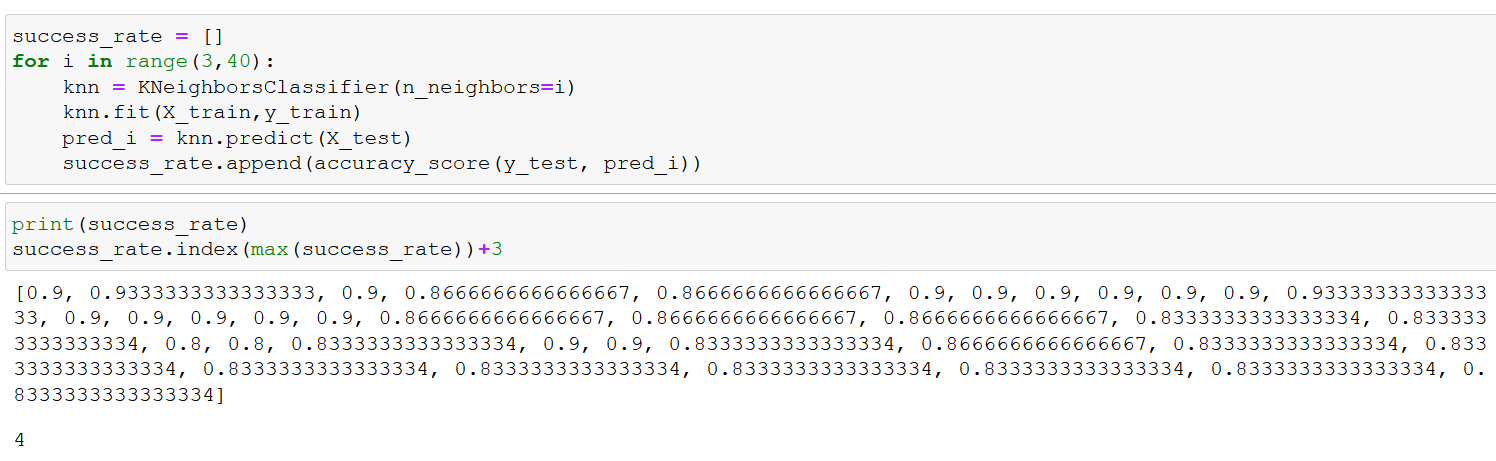
\includegraphics[width=\textwidth]{knnIris.png}
\end{figure}
\FloatBarrier

\noindent The above picture shows that 4 is actually the most optimal value for K as it gives a higher success rate with a train/test split of 80\%/20\%. 



\begin{figure}[!h]
  \caption{KNN Accurracy Score}
  \centering
      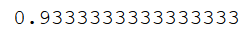
\includegraphics[scale=0.7]{successIris.png}
\end{figure}


\begin{figure}[!h]
  \centering
  \caption{Gaussian Accurracy Score}
    \includegraphics[scale=0.7]{GaussianIris.png}
\end{figure}


\begin{figure}[!h]
  \caption{Multinomial Accurracy Score}
  \centering
    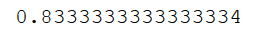
\includegraphics[scale=0.7]{multiIris.png}
\end{figure}

\begin{figure}[!h]
  \caption{Decision Tree Accurracy Score}
  \centering
    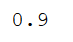
\includegraphics[scale=0.7]{treeIris.png}
\end{figure}
\FloatBarrier

\subsection{Results}
After optimizing and testing each classifier on the dataset, the results suggest that knn is the best classifier for a data set with few attributes and a size of 150 rows. To test our hypothesis, we will take a similar sized dataset and apply the same classifiers to this data. 

\section{Penguin Dataset}
We are using the penguins data set for this experiment. On this dataset we will try to classify which species a penguin is, based on a penguins features. Since the penguins dataset are about double the size of the iris dataset (a little longer actually), we first take a sample of 45\% of the full penguins dataset. This leaves us with 150 entries in the sample, close enough to say that it is similar to the length of the iris dataset.  We can now begin applying the models.
\subsection{Classifiers comparison}
We will be using the same procedure as for the Iris dataset. First find optimal k value, then compute the accuracy scores for the different models.


\begin{figure}[!h]
  \caption{KNN Accurracy Score}
  \centering
      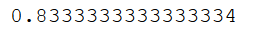
\includegraphics[scale=0.7]{knnPenguin.png}
\end{figure}


\begin{figure}[!h]
  \centering
  \caption{Gaussian Accurracy Score}
    \includegraphics[scale=0.7]{GaussianPenguin.png}
\end{figure}


\begin{figure}[!h]
  \caption{Multinomial Accurracy Score}
  \centering
    
\includegraphics[scale=0.7]{multiPenguin.png}
\end{figure}

\begin{figure}[!h]
  \caption{Decision Tree Accurracy Score}
  \centering
    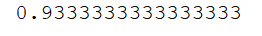
\includegraphics[scale=0.7]{treePenguin.png}
\end{figure}
\FloatBarrier

\subsection{Results}
After testing each classifier on the penguin data, it seems that the hypotheses is incorrect. It was assumed that a similar sized dataset would provide the same results, but the result shows that KNN is not the optimal model in this case. Gaussian Naive Bayes and Decision Tree is more accurate on the penguin dataset.
\section{Wine Quality Dataset}
The last test will be on the wine-quality dataset. It is larger than the iris and penguins dataset combined. Using this dataset, we will try to classify if the wine is red or white, based on the wines physico-chemical content and its quality. Our assumption is that since Decision Tree has performed consistently well on the two previous datasets  (93,3\% on penguins and 90\% on the iris dataset), that it will also perform well on the wine-quality dataset, even though it is of a larger size.
\subsection{Classifiers comparison}
Using the same procedure as for the Iris and Penguins dataset we get:

\begin{figure}[!h]
  \caption{KNN Accurracy Score}
  \centering
      
\includegraphics[scale=0.7]{knnWine.png}
\end{figure}


\begin{figure}[!h]
  \centering
  \caption{Gaussian Accurracy Score}
    \includegraphics[scale=0.7]{GaussianWine.png}
\end{figure}


\begin{figure}[!h]
  \caption{Multinomial Accurracy Score}
  \centering
    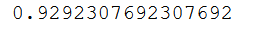
\includegraphics[scale=0.7]{multiWine.png}
\end{figure}

\begin{figure}[!h]
  \caption{Decision Tree Accurracy Score}
  \centering
    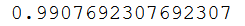
\includegraphics[scale=0.7]{treeWine.png}
\end{figure}
\FloatBarrier

\subsection{Results}
The results from this dataset shows that the decision tree is the most optimal classifier in this case, while Multinomial Naive Bayes continues to be the worst of them all.

\section{Results comparison}
Here is shown the name and score for each model on each dataset (Iris, Penguins, Wine-Quality) and the total average is shown on the right.

\bigskip

\noindent KNN (93,3\%, 83,3\%, 94,9\%)   \hfill            $\approx$ 90,5\%  \\
Gaussian Naive Bayes (83,3\%, 93,3\%, 98\%) \hfill     $\approx$ 91,5\%  \\
Multinomial Naive Bayes (83,3\%, 80\%, 93\%) \hfill     $\approx$ 85,4\% \\
Decision Tree (90,0\%, 93,3\%, 99,1\%) \hfill         $\approx$ 94,1\% \\
\\
From these results it can be seen that Decision Tree performs well in most cases, though it is not the most accurate one in all cases. Worst of all in MultiNomial Naive Bayes which got the lowest score in all cases.

\subsection{Future work}
To further improve upon the results and find the optimal model, we can expand the experiments to include more of the supervised classification models, such as Support Vector Machine and Random Forest.

\section{Conclusion}
The result have proven the hypothesis incorrect. Given our results, we can conclude that there does not exist a single best classifier, though Decision Tree was a viable candidate. We can conclude this because there was no single classifier that had the highest accuracy score on all of the datasets. It is not possible to decide beforehand which one is the most optimal. We conclude that to find the best classifier for your dataset, you have to try different models and see which one provides the best result.


\section{Bibliography}
\nocite{*}
\raggedright
\bibliography{bibliographyClassifier.bib}
\bibliographystyle{plain}
 

\end{document}
